\tableofcontents
\newpage

\section{Цель работы}
По выданному преподавателем варианту восстановить текст заданного варианта программы, определить предназначение и составить описание программы, определить область представления и область допустимых значений исходных данных и результата, выполнить трассировку программы.
\begin{figure}[H]
\centering
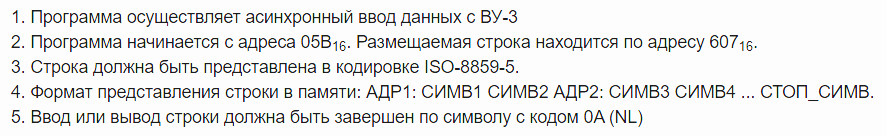
\includegraphics[scale=0.6]{task}
\label{pic:task}
\end{figure}
              
\section{Текст программы}
\noindent
\begin{center}
\begin{tabular}{|c|c|c|l|}
\hline
\multicolumn{1}{|c}{\makecell{\textbf{Адрес}\\\textbf{ячейки}}}
&\multicolumn{1}{|c|}{\makecell{\textbf{Содержимое}\\\textbf{ячейки}}}
&\multicolumn{1}{|c|}{\makecell{\textbf{Мнемоника}}}
&\multicolumn{1}{c|}{\makecell{\textbf{Комментарии}}}\\
\hline
3EA & 03FD & --- & Адрес начала массива \\
3EB & 0200 & --- & Ячейка для хранения адреса обрабатываемого \\
& & & элемента массива \\
3EC & E000 & --- & Ячейка для хранения количества необработанных \\
& & & элементов массива \\
3ED & E000 & --- & Счетчик нечетных элементов \\
\hline
\hline
3EE & 0200 & CLA & Очистка аккумулятора \\
3EF & EEFD & ST (IP - 3) & Сохраняем аккумулятор в ячейку 0x3ED \\
\hline
3F0 & AF05 & LD \#0x5 & Загружаем \#0x5 в аккумулятор \\
3F1 & EEFA & ST (IP - 6) & Сохраняем аккумулятор в ячейку 0x3EC \\
\hline
3F2 & AEF7 & ADD (IP - 9) & Складываем аккумулятор с элементом в 0x3EA \\
3F3 & EEF7 & ST (IP - 9) & Сохраняем аккумулятор в ячейку 0x3EB \\
\hline
3F4 & ABF6 & LD - (IP - 10) & Загружаем элемент  массива по \\
& & & адресу в ячейке 0x3EB \\
3F5 & 0480 & ROR & Циклический сдвиг вправо \\
3F6 & F401 & BLO BCS (IP + 2) & Если C равно 1, то будет осуществлен \\
& & & переход в 0x3F8 (0x3F8 -> IP) \\
3F7 & CE02 & BR JUMP (IP + 3) & Безусловный переход в 0x3FA \\
3F8 & 0400 & ROL & Циклический сдвиг влево \\
3F9 & 6AF3 & ADD (L)+ (IP - 13) & Косвенная автоинкрементная адресация 0x3ED \\
3FA & 83EC & LOOP 0x3EC & Декремент и пропуск. Если MEM(0x3EC) $\leq$ 0, \\
& & & то IP + 1 -> IP \\
3FB & CEF8 & BR (IP - 8) & Безусловный переход в 0x3F4 \\
3FC & 0100 & HLT & Остановка \\
\hline
\hline
3FD & 0740 & --- & \\
3FE & 0B01 & --- & \\
3FF & 0E01 & --- & Элементы массива \\
400 & E3EF & --- & \\
401 & 0E01 & --- & \\
\hline
\end{tabular}
\end{center}

\section{Описание программы}
\subsection{Назначение программы и реализуемая ею функция (формула)}
\subsection*{Назначение программы}
\noindent Программа подсчитывает количество нечетных элементов массива.

\subsection*{Реализуемая функция (формула)}

\noindent $Y=\sum_{i=1}^{5} X_{i} \text { mod } 2$

\subsection{Область представления и область допустимых значений исходных данных и результата}

\subsection*{Область представления}
\noindent
Исходные данные: \\
Aдрес начала массива (3EA): 11-разрядные беззнаковые числа, с фиксированной запятой.\\
Диапазон значений: $0\ldots2^{11}-1$ \\
Элементы массива (3FD--401): 16-разрядные знаковые числа, фиксированной запятой.\\
Диапазон значений:  $-2^{15}\ldots2^{15}-1$ \\\\
Результат: \\
Счетчик нечетных элементов (3ED): 16-разрядное беззнаковое число, фиксированной запятой.\\
Диапазон значений:  $0\ldots2^{15}-1$

\subsection*{Область допустимых значений}
\noindent Исходные данные: \\
Aдрес начала массива (3EA): [000, 3E5] $\cup$ [3FD, 7FF] \\
Элементы массива (3FD--401): совпадает с областью представления\\\\
Результат: \\
Счетчик нечетных элементов (3ED): $0\ldots5$

\subsection{Расположение в памяти ЭВМ программы, исходных данных и результатов}
\noindent Программа: 3EE--3FC \\
Исходные данные: \\
Aдрес начала массива: 3EA (Z $=$ Содержимое ячейки 3EA) \\
Элементы массива: 3FD--401 (Z--(Z$+$4), элемент массива: $X_{i}$) \\
Вспомогательные ячейки: 3EB, 3EC \\
Результат: 3ED (Y $=$ Содержимое ячейки 3ED)

\subsection{Адреса первой и последней выполняемой команд программы}
\noindent Адрес первой выполняемой команды : 3EE \\
Адрес последней выполняемой команды: 3FC

\section{Таблица трассировки}
\begin{flushleft}
\begin{tabular}{|c|c|c|c|c|c|c|c|c|c|c|c|}
\hline
\multicolumn{2}{|c}{\makecell{\textbf{Выполняемая}\\\textbf{команда}}}
  &\multicolumn{8}{|c|}{\textbf{Содержимое регистров после выполнения команды}}
  &\multicolumn{2}{c|}{\makecell{\textbf{Ячейка, }\\\textbf{содержимое}\\\textbf{которой}\\\textbf{изменилось}}}\\
\hline
Адрес & Код & IP & CR & AR & DR & SP & BR & AC & NZVC & Адрес & Новый код\\
\hline
3EE & 0200 & 3EF & 0200 & 3EE & 0200 & 000 & 03EE & 0000 & 0100 & --- & ---
\\
\hline
3EF & EEFD & 340 & EEFD & 3ED & 0000 & 000 & FFFD & 0000 & 0100 & 3ED & 0000
\\
\hline
3F0 & AF05 & 3F1 & AF05 & 3F0 & 0005 & 000 & 0005 & 0005 & 0000 & --- & ---
\\
\hline
3F1 & EEFA & 3F2 & EEFA & 3EC & 0005 & 000 & FFFA & 0005 & 0000 & 3EC & 0005
\\
\hline
3F2 & 4EF7 & 3F3 & AEF7 & 3EA & 03FD & 000 & FFF7 & 03FD & 0000 & --- & ---
\\
\hline
3F3 & EEF7 & 3F4 & EEF7 & 3EB & 03FD & 000 & FFF7 & 03FD & 0000 & 3EB & 03FD
\\
\hline
\hline
3F4 & ABF6 & 3F5 & AAF6 & 3FD & 0740 & 000 & FFF6 & 0740 & 0000 & 3EB & 03FE
\\
\hline
3F5 & 0480 & 3F6 & 0480 & 3F5 & 0480 & 000 & 03F5 & 03A0 & 0000 & --- & ---
\\
\hline
3F6 & F401 & 3F7 & F401 & 3F6 & F401 & 000 & 03F6 & 03A0 & 0000 & --- & ---
\\
\hline
3F7 & CE02 & 3FA & CE02 & 3F7 & 03FA & 000 & 0002 & 03A0 & 0000 & --- & ---
\\
\hline
3FA & 83EC & 3FB & 83EC & 3EC & 0003 & 000 & 03FA & 03A0 & 0000 & 3EC & 0004
\\
\hline
3FB & CEF8 & 3F4 & CEF8 & 3FB & 03F4 & 000 & FFF8 & 03A0 & 0000 & --- & ---
\\
\hline
\hline
3F4 & ABF6 & 3F5 & AAF6 & 3FE & 0B01 & 000 & FFF6 & 0B01 & 0000 & 3EB & 03FF
\\
\hline
3F5 & 0480 & 3F6 & 0480 & 3F5 & 0480 & 000 & 03F5 & 0580 & 0000 & --- & ---
\\
\hline
3F6 & F401 & 3F8 & F401 & 3F6 & F401 & 000 & 0001 & 0580 & 0011 & --- & ---
\\
\hline
3F8 & 0400 & 3F9 & 0400 & 3F8 & 0400 & 000 & 03F1 & 0B01 & 0000 & --- & ---
\\
\hline
3F9 & 6AF3 & 3FA & 6AF3 & 000 & 0000 & 000 & FFF3 & 0B01 & 0001 & 3ED & 0001
\\
\hline
3FA & 83EC & 3FB & 83EC & 3EC & 0002 & 000 & 03FA & 0B01 & 0001 & 3EC & 0003
\\
\hline
3FB & CEF8 & 3F4 & CEF8 & 3FB & 03F4 & 000 & FFF8 & 0B01 & 0001 & --- & ---
\\
\hline
\hline
3F4 & ABF6 & 3F5 & AAF6 & 3FF & 0E01 & 000 & FFF6 & 0E01 & 0001 & 3EB & 0400
\\
\hline
3F5 & 0480 & 3F6 & 0480 & 3F5 & 0480 & 000 & 03F5 & 8700 & 1001 & --- & ---
\\
\hline
3F6 & F401 & 3F8 & F401 & 3F6 & F401 & 000 & 0001 & 8700 & 1001 & --- & ---
\\
\hline
3F8 & 0400 & 3F9 & 0400 & 3F8 & 0400 & 000 & 03F8 & 0E01 & 0011 & --- & ---
\\
\hline
3F9 & 6AF3 & 3FA & 6AF3 & 0001 & 0000 & 000 & FFF3 & 0E01 & 0001 & 3ED & 0002
\\
\hline
3FA & 83EC & 3FB & 83EC & 3EC & 0001 & 000 & 03FA & 0E01 & 0001 & 3EC & 0002
\\
\hline
3FB & CEF8 & 3F4 & CEF8 & 3FB & 03F4 & 000 & FFF8 & 0E01 & 0001 & --- & ---
\\
\hline
\hline
3F4 & ABF6 & 3F5 & AAF6 & 400 & E3EF & 000 & FFF6 & E3EF & 1001 & 3EB & 0401
\\
\hline
3F5 & 0480 & 3F6 & 0480 & 3FA & 0480 & 000 & 03F5 & F1F7 & 1001 & --- & ---
\\
\hline
3F6 & F401 & 3F8 & F401 & 3F6 & F401 & 000 & 0001 & F1F7 & 1001 & --- & ---
\\
\hline
3F8 & 0400 & 3F9 & 0400 & 3F8 & 0400 & 000 & 03F8 & E3EF & 1001 & --- & ---
\\
\hline
3F9 & 6AF3 & 3FA & 6AF3 & 002 & 0000 & 000 & FFF3 & E3EF & 1001 & 3ED & 0003
\\
\hline
3FA & 83EC & 3FB & 83EC & 3EC & 0000 & 000 & 03FA & E3EF & 1001 & 3EC & 0001
\\
\hline
3FB & CEF8 & 3F4 & CEF8 & 3FB & 03F4 & 000 & FFF8 & E3EF & 1001 & --- & ---
\\
\hline
\hline
3F4 & ABF6 & 3F5 & AAF6 & 401 & 0E01 & 000 & FFF6 & 0E01 & 0001 & 3EB & 0402
\\
\hline
3F5 & 0480 & 3F6 & 0480 & 3F5 & 0480 & 000 & 03F5 & 8700 & 1001 & --- & ---
\\
\hline
3F6 & F401 & 3F8 & F401 & 3F6 & F401 & 000 & 0001 & 8700 & 1001 & --- & ---
\\
\hline
3F8 & 0400 & 3F9 & 0400 & 3F8 & 0400 & 000 & 03F8 & 0E01 & 0011 & --- & ---
\\
\hline
3F9 & 6AF3 & 3FA & 6AF3 & 003 & 0000 & 000 & FFF3 & 0E01 & 0001 & 3ED & 0004
\\
\hline
3FA & 83EC & 3FC & 83EC & 0E01 & FFFF & 000 & 03FA & 0E01 & 0001 & 3EC & 0000
\\
\hline
\hline
3FC & 0100 & 3FD & 0100 & 3FC & 0100 & 000 & 3FC & 001B & 0000 & --- & --- \\
\hline
\end{tabular}
\end{flushleft}

\section{Диапазон всех ячеек памяти, где может размещаться массив исходных данных}
Диапазон: [000, 3E5] $\cup$ [3FD, 7FF]

\section{Вывод}
В ходе выполнения данной лабораторной работы я познакомился с режимами адресации БЭВМ и новыми для меня командами - ветвления, сравнения, командой LOOP. На практике разобрался с циклом выборки адреса для разных режимов адресации.